\subsection{Doble recubrimiento}
	\label{sec:function_5}
	
	Para evitar que una formación colisione con otra formación que se encuentre detenida más adelante en la misma vía o circulando a menor velocidad, el sistema de enclavamiento deberá controlar las señales entre ambas para regular la velocidad y distancia entre ellas. Tal como se explicó en la Sección \ref{sec:signals}, las señales pueden presentar diferentes aspectos. Cada aspecto determinará un rango de velocidad permitido, siendo rojo el mas restrictivo. La Figura \ref{fig:ACG_recrubrimiento_1} ilustra el comportamiento del señalamiento cuando dos formaciones circulan en el mismo sentido, separadas por una distancia de seguridad.
	
	\begin{figure}[!h]
		\centering
		\includegraphics[width=1\textwidth]{Figuras/recubrimiento}
		\centering\caption{Protección por doble recubrimiento.}
		\label{fig:ACG_recrubrimiento_1}
	\end{figure}
	
	La formación que circula por detrás (formación A en la Figura \ref{fig:ACG_recrubrimiento_1}) se encuentra frente a una señal de aspecto verde, por lo
	que puede continuar su marcha sin restricciones, siempre y cuando su velocidad sea menor a la velocidad máxima permitida en la red ferroviaria. Si la formación A reduce la distancia a la formación B, pasará a estar regida por una señal de aspecto amarillo. Si esto sucediera, la formación A deberá disminuir su velocidad para volver a situarse dentro de una sección verde. Lo mismo ocurriría si la formación A alcanzara una señal de aspecto doble amarillo, indicada mediante la señal naranja en la Figura 3.8. En este caso dado que la distancia entre formaciones es aún menor, deberá reducirse aún más la velocidad.
	
	Si la formación A continúa con una mayor velocidad que la formación B, la distancia entre ambas se reducirá y el señalamiento que la formación A tiene en su camino le impondrá velocidades más y más reducidas, hasta que la distancia entre ambas formaciones se incremente a un valor seguro.
		
	Debido al bloqueo por ocupación, todas las secciones ocupadas por una formación presentan una señal a peligro (roja). Inmediatamente detrás de cada formación se genera una secuencia de señales denominada doble recubrimiento. Si la formación avanza y cambia de sección, las señales de protección cambiarán su aspecto acorde al movimiento de la formación, de forma tal que siempre la sección donde está la formación tenga su señal de protección en rojo, la sección anterior en amarillo, la sección anterior en doble amarillo y la sección anterior en verde. Si no hay ninguna formación en la sección anterior a la que tiene su señal en verde, entonces esa sección también tendrá su señal en verde, lo mismo que todas las secciones anteriores, hasta que haya una formación que ocupe una sección, en cuyo caso esa sección estará en rojo y la secuencia de doble recubrimiento se repetirá también detrás de esa formación.
	 
	La cantidad de señales y la secuencia de aspectos variará según el operador de la red, las normas locales o nacionales. Algunos países como el Reino Unido \cite{UK} utilizan la secuencia rojo-doble amarillo-amarillo-verde (Figura \ref{fig:uk_signalling}) y esta es la secuencia de aspectos que implementa el ACG en este trabajo, aunque cabe aclarar que el ACG puede modificarse para implementar otras secuencias. 
	
	\begin{figure}[!h]
		\centering
		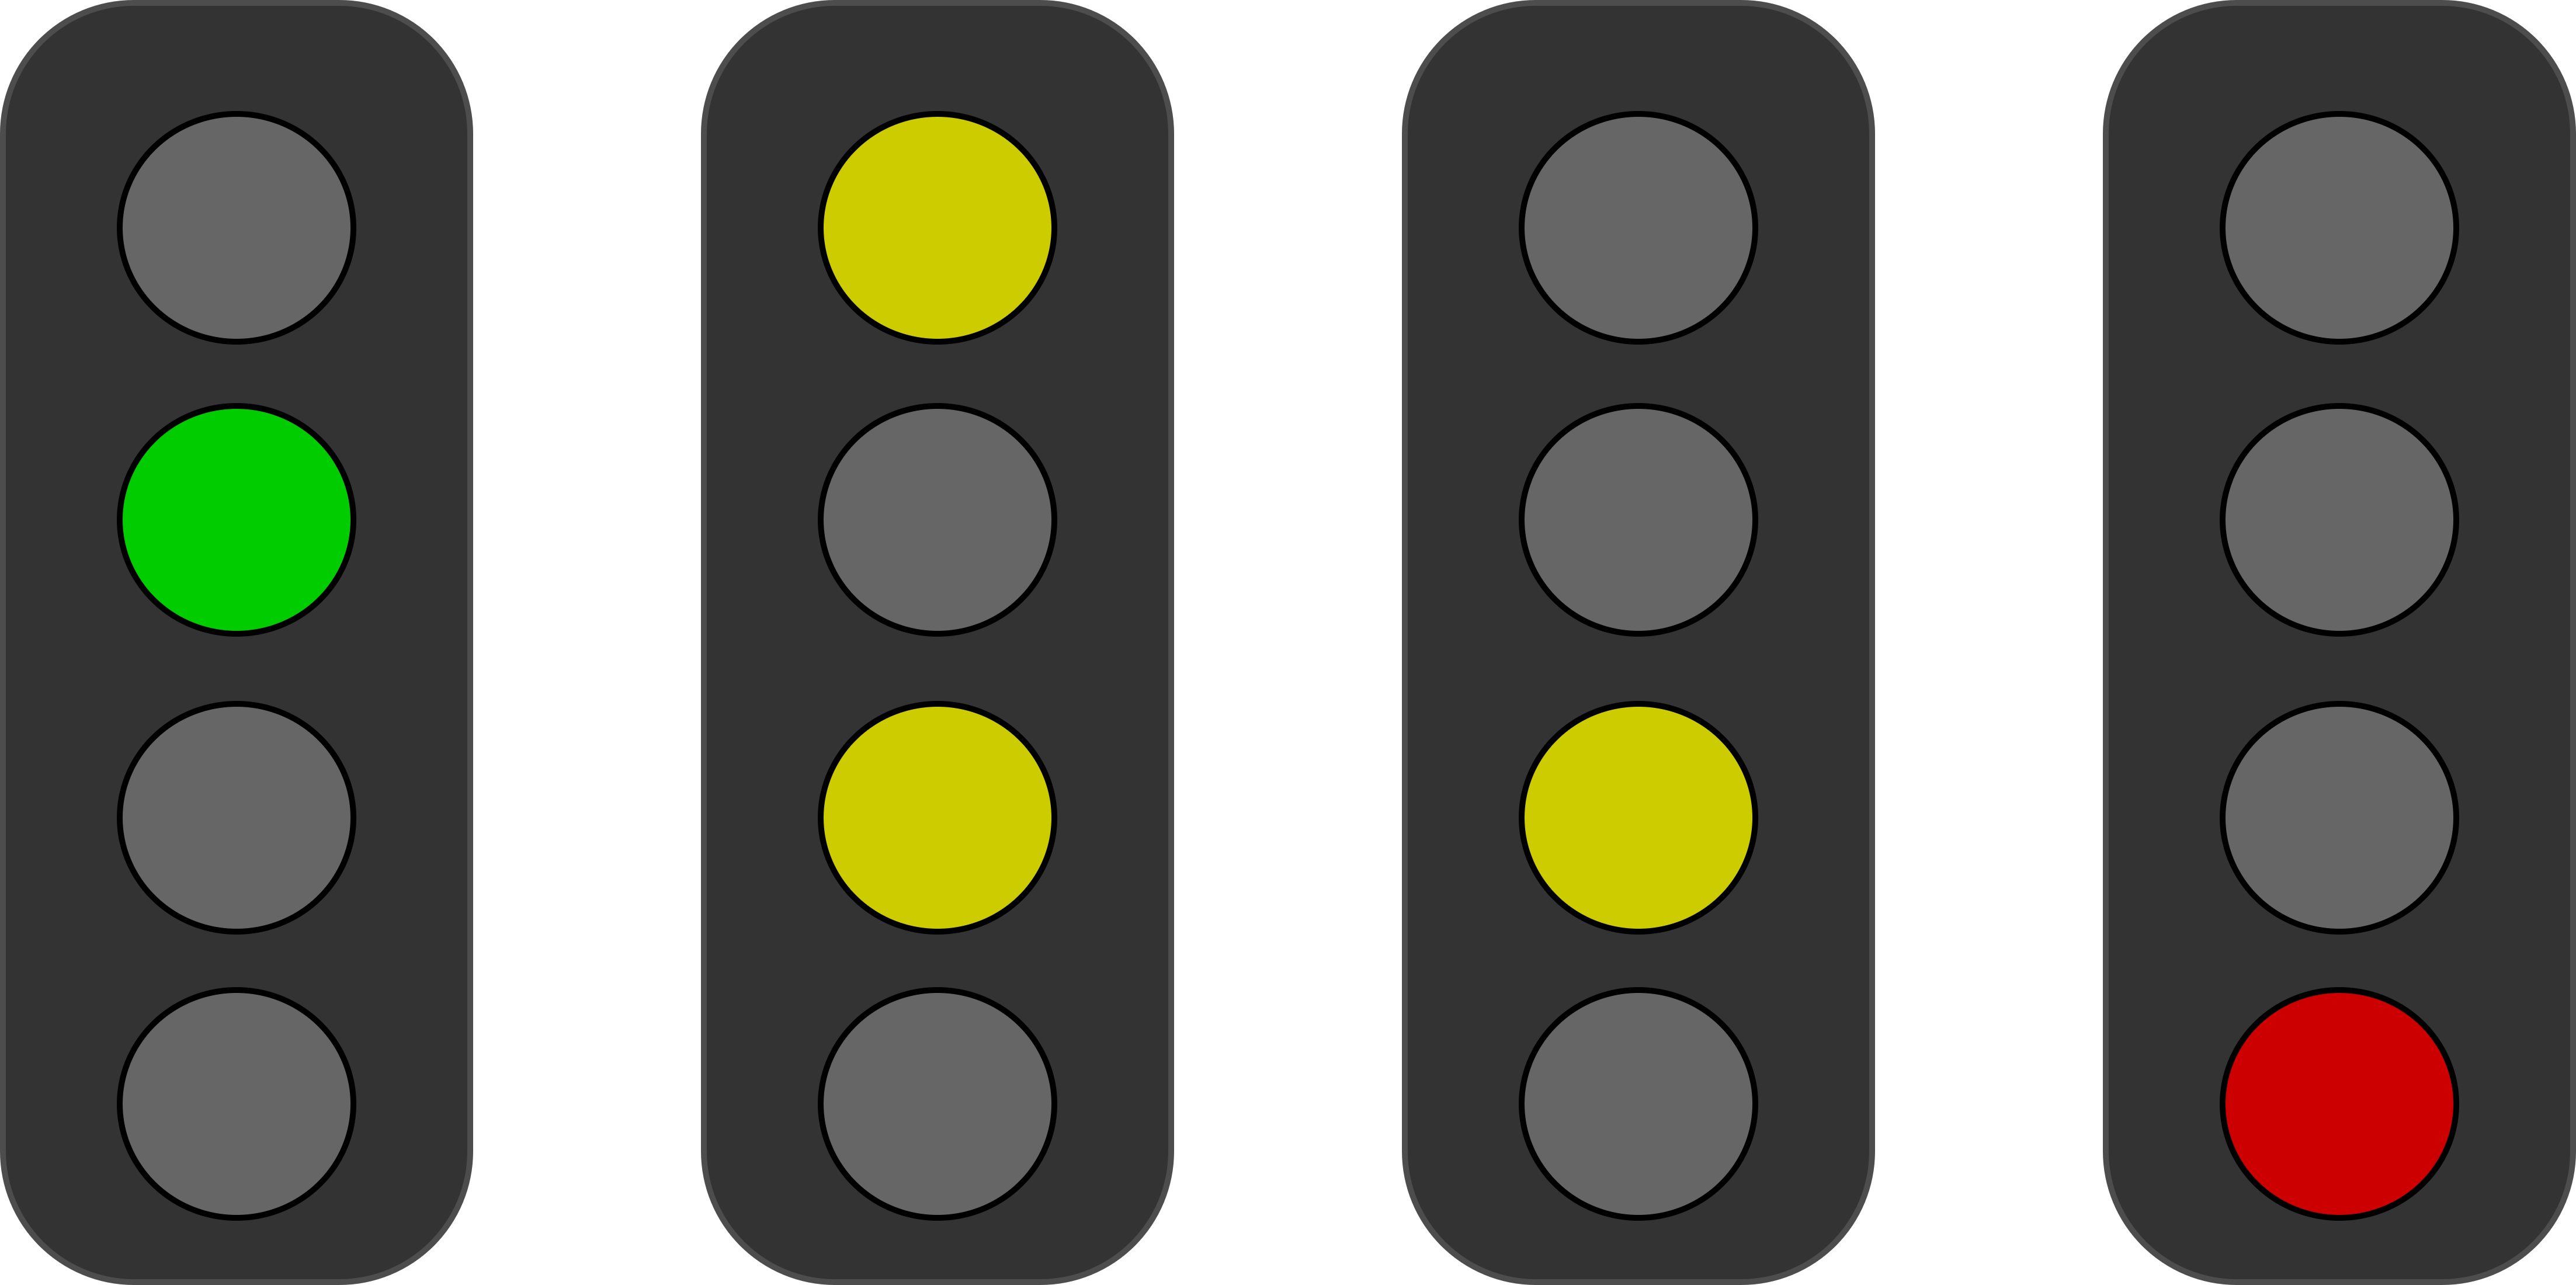
\includegraphics[width=0.5\textwidth]{Figuras/semaforo2}
		\centering\caption{Protección por doble recubrimiento.}
		\label{fig:uk_signalling}
	\end{figure}
	
	En las etapas iniciales del proyecto la única herramienta de visualización era Design4Rail \cite{DESIGN4RAIL}. Esta herramienta solamente puede representar señales de un aspecto y, al no tener todavía implementado el AGG, no era posible representar señales de doble aspecto amarillo. Es por esa razón que el RNA reemplazó la señal doble amarilla por una señal naranja. Este reemplazo también es realizado por el ACG al implementar las señales en VHDL. El proyecto se encontraba en estado muy avanzado cuando se diseñó el AGG, por lo que se mantuvo que todas las señales son de un único aspecto. En este trabajo, por lo tanto, siempre se representará mediante una señal naranja a una señal doble amarilla.
	
	
	%Ya que Design4Rail \cite{DESIGN4RAIL}, el software utilizado para visualizar el señalamiento al inicio del proyecto, solo puede representar señales de un aspecto, en la Figura \ref{fig:ACG_recrubrimiento_1} se reemplazó la señal doble amarilla por una señal naranja. En este trabajo siempre se representará mediante una señal naranja a una señal doble amarilla.

	
	